\chapter{Adaptieve afweer en vaccinatie}\label{ch:b3:adaptive-immunity}

In 1796 kraste een plattelandsarts pus uit de koepokzweer van een
melkmeisje in de arm van een jongen en entte hem zes weken later met
pokken; de jongen werd niet ziek. In 1980 verklaarde de
Wereldgezondheidsorganisatie de pokken --- die in de twintigste eeuw
driehonderd miljoen mensen hadden gedood --- met die methode van de
aarde uitgeroeid. Het stelsel dat Jenner had ingeschakeld zonder te
weten dat het bestond, herkent elk molecuul dat het nooit eerder heeft
ontmoet, kiest uit honderd miljard verschillende receptoren de weinige
die passen, vermenigvuldigt de cellen die deze dragen in een week
miljoenvoudig, verbetert ondertussen hun pasvorm door mutatie en
selectie, en onthoudt de uitkomst een leven lang; het leert ook het
lichaam dat het heeft voortgebracht niet aan te vallen, en waar dat
leren mislukt ontstaan de auto-immuunziekten. Dit hoofdstuk behandelt
de \omterm{def:b3:adaptive-immunity:lymphocytes}{lymfocyten} en hoe zij hun receptoren maken, hoe een afweerreactie op
gang komt en wordt onthouden, hoe \omterm{def:b3:adaptive-immunity:tolerance}{tolerantie} wordt afgedwongen en
verloren gaat, en de rekenkunde waarmee het vaccineren van genoeg
mensen ook hen beschermt die niet zijn gevaccineerd.

\section{Lymfocyten en klonale selectie}

\begin{definition}[Lymfocyten en hun receptoren]\label{def:b3:adaptive-immunity:lymphocytes}
\index{lymfocyt}\index{B-cel}\index{T-cel}\index{antigeen}\index{klonale selectie}\index{lymfeknoop}
\emph{Adaptieve afweer} berust op \emph{lymfocyten}: \emph{B-cellen},
die in het beenmerg rijpen en wier antigeenreceptor een
membraangebonden \emph{\omterm{def:b3:adaptive-immunity:antibody}{antilichaam}} is dat zij later uitscheiden; en
\emph{T-cellen}, die in de \omterm{def:b3:adaptive-immunity:tolerance}{thymus} rijpen en wier receptor
peptidefragmenten herkent die op het oppervlak van andere cellen worden
getoond. Een \emph{antigeen} is alles wat een receptor bindt; het deel
dat werkelijk wordt geraakt is een \emph{epitoop}. Het grondfeit is de
\emph{klonale selectie} (Burnet, 1957): elke lymfocyt draagt receptoren
van slechts één specificiteit, vastgelegd voordat hij enig antigeen
ontmoet; het lichaam houdt een repertoire van zo'n $10^{11}$ van zulke
cellen aan; een antigeen selecteert de weinige cellen wier receptoren
passen en drijft ze tot deling in een kloon van effector- en
\omterm{def:b3:adaptive-immunity:response}{geheugencellen}; en lymfocyten wier receptoren op de eigen moleculen van
het lichaam passen worden tijdens hun rijping verwijderd of stilgelegd.
De cellen circuleren voortdurend tussen het bloed en de
\emph{lymfeknopen}, de milt en het lymfoïde weefsel van de slijmvliezen,
waar antigeen wordt getoond dat door \omterm{def:b3:innate-immunity:innate}{dendritische cellen} is aangevoerd
(\cref{ch:b3:innate-immunity}), zodat de zeldzame passende cel --- één
op honderdduizend voor een gegeven epitoop --- het binnen een dag of
twee vindt.
\end{definition}

\begin{proof}[Bewijsmateriaal]
Nossal en Lederberg (1958) brachten afzonderlijke \omterm{def:b3:adaptive-immunity:lymphocytes}{lymfocyten} uit
geïmmuniseerde ratten in microdruppels en toetsten het \omterm{def:b3:adaptive-immunity:antibody}{antilichaam} dat
elk van hen uitscheidde: elke cel maakte \omterm{def:b3:adaptive-immunity:antibody}{antilichaam} tegen één van de
twee antigenen, nooit tegen beide. Burnet had het het jaar tevoren
voorspeld. Tonegawa (1976) vergeleek het DNA van een antilichaamgen in
embryonale cellen en in een \omterm{def:b3:adaptive-immunity:antibody}{antilichaam} uitscheidende \omterm{def:b3:cancer-biology:hallmarks}{tumor}: in het
embryo lagen het variabele en het constante deel ver uiteen, in de
\omterm{def:b3:cancer-biology:hallmarks}{tumor} waren ze aaneengevoegd --- het gen was in de somatische cel
geknipt en geplakt, de eerste demonstratie van een genoom dat met opzet
is herschikt.
\end{proof}

\section{Honderd miljard receptoren maken}

\begin{definition}[Bouw van het antilichaam en V(D)J-recombinatie]\label{def:b3:adaptive-immunity:antibody}
\index{antilichaam}\index{immunoglobuline}\index{V(D)J-recombinatie}\index{RAG}\index{junctionele diversiteit}\index{klassenwisseling}
Een \emph{antilichaam} (immunoglobuline) bestaat uit twee identieke
zware ketens en twee identieke lichte ketens, elk met een
\emph{variabel} domein aan het uiteinde en \emph{constante} domeinen
erachter; de twee armen binden elk een epitoop via drie hypervariabele
lussen van het zware en drie van het lichte variabele domein, en de
stam (Fc) is wat fagocyten, \omterm{def:b3:innate-immunity:complement}{complement} en mestcellen herkennen. Vijf
klassen verschillen in het constante deel van hun zware keten: IgM, het
eerst gemaakte, een pentameer dat \omterm{def:b3:innate-immunity:complement}{complement} goed activeert; IgG, het
werkpaard van bloed en weefsels, dat de placenta passeert; IgA, een
dimeer dat over de slijmvliezen naar darm, luchtwegen en melk wordt
uitgescheiden; IgE, gebonden door mestcellen, tegen wormen --- en de
oorzaak van allergie; IgD. De variabele domeinen zijn als zodanig niet
gecodeerd. De zware-ketenlocus bevat ongeveer $40$ werkzame
\emph{V}-segmenten, $25$ \emph{D}- en $6$ \emph{J}-segmenten; een
\omterm{def:b3:adaptive-immunity:lymphocytes}{B-cel} in ontwikkeling kiest er van elk één en voegt ze samen door
\emph{V(D)J-recombinatie}: de enzymen RAG1 en RAG2 knippen bij de
recombinatiesignaalsequenties die de segmenten flankeren, en de
uiteinden worden samengevoegd door de niet-homologe
eindverbindingsmachinerie van \cref{ch:b3:dna-repair}, waarbij bij elke
naad willekeurig nucleotiden worden weggeknipt en toegevoegd (door het
enzym TdT) --- \emph{junctionele diversiteit}, die precies in de derde
hypervariabele lus valt. De lichte ketens doen hetzelfde met V en J.
Nadat de afweerreactie is begonnen wordt hetzelfde variabele domein
door een tweede herschikking aan een ander constant deel gekoppeld, de
\emph{klassenwisseling}, die de functie van het antilichaam verandert
maar niet zijn specificiteit.
\end{definition}

\begin{theorem}[De omvang van het repertoire]\label{thm:b3:adaptive-immunity:repertoire}
\index{repertoire!combinatorisch}
Met $V_{H} = 40$, $D = 25$, $J_{H} = 6$ zware segmenten, en lichte
ketens uit twee loci met $(V_{\kappa}, J_{\kappa}) = (40, 5)$ en
$(V_{\lambda}, J_{\lambda}) = (30, 4)$, bedraagt het aantal
verschillende combinaties van zware en lichte keten die alleen al door
segmentkeuze bereikbaar zijn
\[
(40\times 25\times 6)\times(40\times 5 + 30\times 4) = 6000\times 320
= 1.9\times 10^{6}.
\]
\omterm{def:b3:adaptive-immunity:antibody}{Junctionele diversiteit} bij de twee zware naden en de ene lichte naad
vermenigvuldigt dit met een factor van de orde $10^{4}$--$10^{5}$, wat
een mogelijk repertoire van meer dan $10^{10}$ oplevert uit minder dan
$200$ gensegmenten --- meer dan het aantal B-cellen in een lichaam,
zodat het werkelijke repertoire een steekproef uit het mogelijke is.
\omterm{def:b3:adaptive-immunity:germinal-centre}{Somatische hypermutatie} tijdens de afweerreactie (hieronder) brengt
daarna varianten van elke geselecteerde receptor voort.
\end{theorem}
\begin{proof}
Elke zware keten is één V, één D en één J; elke lichte keten één V en
één J uit een van beide loci; elke zware keten paart met elke lichte,
dus vermenigvuldigen de aantallen zich (vermenigvuldigingsregel), en de
twee lichte loci tellen op. De junctionele factor is het aantal
verschillende sequenties dat het willekeurige wegknippen en toevoegen
bij een naad kan opleveren --- minstens enkele tientallen per naad ---
verheven tot het aantal naden; zijn precieze waarde ligt niet vast,
maar drie naden met elk $30$--$50$ uitkomsten geven $3\times 10^{4}$
tot $10^{5}$. Het aantal voor \omterm{def:b3:adaptive-immunity:mhc}{T-celreceptoren}, met twee ketens die op
dezelfde wijze worden herschikt en een grotere junctionele bijdrage, is
van dezelfde orde.
\end{proof}

\begin{omfigure}
\begin{tikzpicture}[every node/.style={font=\scriptsize}, >=stealth]
  % antibody Y
  \begin{scope}[xshift=0cm]
    % heavy chains
    \draw[very thick, omDef] (0,0) -- (0,1.6) -- (-1.3,3.0); \draw[very thick, omDef] (0.35,0) -- (0.35,1.6) -- (1.65,3.0);
    % light chains
    \draw[very thick, omProp] (-0.45,1.55) -- (-1.75,2.95); \draw[very thick, omProp] (0.8,1.55) -- (2.1,2.95);
    \fill[omThm] (-1.55,3.0) circle (0.12); \fill[omThm] (1.9,3.0) circle (0.12);
    \node[above, align=center] at (-1.5,3.15) {variabele domeinen:\\antigeenbindingsplaats}; 
    \node[right, align=left] at (0.55,0.5) {Fc-stam (constant):\\de klasse bepaalt de functie};
    \node[left, omProp] at (-0.7,2.1) {licht}; \node[right, omDef] at (0.4,1.3) {zwaar};
    \draw[omDef] (0.05,1.1) -- (0.3,1.1); \draw[omDef] (0.05,0.7) -- (0.3,0.7);
  \end{scope}
  % V(D)J locus
  \begin{scope}[xshift=4.2cm, yshift=2.4cm, xscale=0.86]
    \draw[very thick, gray] (0,0) -- (8.2,0);
    \foreach \x in {0.2,0.6,1.0,1.4} \draw[thick, fill=omDef!40] (\x,-0.15) rectangle (\x+0.3,0.15);
    \node[above] at (0.95,0.2) {V-segmenten ($\sim 40$)}; \node[font=\tiny] at (1.95,0) {$\cdots$};
    \foreach \x in {2.5,2.8,3.1} \draw[thick, fill=omProp!50] (\x,-0.15) rectangle (\x+0.2,0.15);
    \node[above] at (2.9,0.2) {D ($25$)};
    \foreach \x in {3.8,4.1,4.4} \draw[thick, fill=omMeth!50] (\x,-0.15) rectangle (\x+0.2,0.15);
    \node[above] at (4.2,0.2) {J ($6$)};
    \foreach \x/\lab in {5.3/\mu,6.0/\delta,6.7/\gamma,7.4/\alpha} { \draw[thick, fill=gray!30] (\x,-0.15) rectangle (\x+0.5,0.15); \node[above] at (\x+0.25,0.2) {C$_{\lab}$}; }
    \draw[->, thick] (4.1,-0.4) -- (4.1,-1.1) node[midway, right, align=left, font=\tiny] {RAG knipt bij de signaalsequenties;\\één V, één D en één J worden\\samengevoegd, TdT voegt\\willekeurige nucleotiden toe};
    % rearranged
    \draw[very thick, gray] (0,-1.5) -- (3.3,-1.5);
    \draw[thick, fill=omDef!40] (1.0,-1.65) rectangle (1.3,-1.35); \fill[omThm] (1.3,-1.65) rectangle (1.4,-1.35);
    \draw[thick, fill=omProp!50] (1.4,-1.65) rectangle (1.6,-1.35); \fill[omThm] (1.6,-1.65) rectangle (1.7,-1.35);
    \draw[thick, fill=omMeth!50] (1.7,-1.65) rectangle (1.9,-1.35);
    \draw[thick, fill=gray!30] (2.6,-1.65) rectangle (3.1,-1.35); \node[above] at (2.85,-1.3) {C$_{\mu}$};
    \node[below, align=center] at (1.45,-1.7) {VDJ samengevoegd: het variabele domein,\\rood: junctionele nucleotiden};
    \node[right, align=left, font=\tiny] at (3.4,-2.0) {gekoppeld aan C$_{\mu}$:\\een zware IgM-keten;\\klassenwisseling verbindt\\later dezelfde VDJ met\\C$_{\gamma}$ of C$_{\alpha}$};
  \end{scope}
\end{tikzpicture}

{\small Links: een \omterm{def:b3:adaptive-immunity:antibody}{antilichaam} --- twee zware en twee lichte ketens,
met de variabele domeinen aan de punten, die twee bindingsplaatsen
vormen, en de constante stam die de rest van het afweersysteem afleest.
Rechts: de zware-ketenlocus voor en na \omterm{def:b3:adaptive-immunity:antibody}{V(D)J-recombinatie}, die van elke
soort één segment kiest en bij de naden willekeurige nucleotiden
toevoegt.}
\end{omfigure}

\begin{definition}[T-celreceptoren en MHC]\label{def:b3:adaptive-immunity:mhc}
\index{T-celreceptor}\index{belangrijkste weefselverenigbaarheidscomplex}\index{antigeenpresentatie}\index{MHC-restrictie}\index{HLA}
De \emph{T-celreceptor} is een molecuul van twee ketens, gebouwd door
dezelfde recombinatie, dat nooit wordt uitgescheiden en geen \omterm{def:b3:adaptive-immunity:lymphocytes}{antigeen}
bindt dat vrij in oplossing is: hij herkent een kort peptide in de
groeve van een molecuul van het \emph{belangrijkste
weefselverenigbaarheidscomplex} (MHC) op het oppervlak van een andere
cel. \emph{MHC-klasse~I}, op elke kernhoudende cel, toont peptiden van
acht tot tien residuen die het proteasoom uit de eigen cytosolische
eiwitten van de cel heeft geknipt --- een steekproef van wat de cel
maakt, met inbegrip van elk \omterm{def:b3:virology:virus}{virus} --- aan \emph{CD8}-T-cellen, die de
cel doden als het peptide vreemd is. \emph{MHC-klasse~II}, op
\omterm{def:b3:innate-immunity:innate}{dendritische cellen}, \omterm{def:b3:innate-immunity:innate}{macrofagen} en B-cellen, toont peptiden van dertien
tot vijfentwintig residuen uit eiwitten die de cel heeft opgenomen en
in endosomen verteerd, aan \emph{CD4}-T-cellen, die met hulp
antwoorden. Een \omterm{def:b3:adaptive-immunity:lymphocytes}{T-cel} is \emph{gerestricteerd}: hij herkent zijn
peptide alleen op het MHC-allel waarop hij is geselecteerd. De MHC-genen
(\emph{HLA} bij de mens) zijn de meest polymorfe van het genoom, met
duizenden allelen die elk in de groeve verschillen, zodat ieder mens
een andere steekproef van de peptiden van elk eiwit toont en geen
ziekteverwekker bij iedereen aan presentatie ontsnapt --- en zodat een
getransplanteerd orgaan van een niet-passende donor door een groot deel
van de T-cellen van de ontvanger als vreemd wordt herkend.
\end{definition}

\begin{proof}[Bewijsmateriaal]
Zinkernagel en Doherty (1974) besmetten muizen van twee ingeteelde
stammen met een \omterm{def:b3:virology:virus}{virus} en toetsten hun cytotoxische T-cellen op
besmette doelcellen: de T-cellen doodden besmette cellen van hun eigen
stam maar niet van de andere, hoewel het \omterm{def:b3:virology:virus}{virus} hetzelfde was. De \omterm{def:b3:adaptive-immunity:lymphocytes}{T-cel}
zag het \omterm{def:b3:virology:virus}{virus} alleen samen met een eigen MHC-molecuul ---
\emph{\omterm{def:b3:adaptive-immunity:mhc}{MHC-restrictie}} --- wat later werd verklaard toen de
kristalstructuur van een MHC-molecuul (Bjorkman, 1987) een groeve met
een peptide erin liet zien, en werd aangetoond dat de \omterm{def:b3:adaptive-immunity:mhc}{T-celreceptor} die
twee samen bindt.
\end{proof}

\begin{omfigure}
\begin{tikzpicture}[every node/.style={font=\scriptsize}, >=stealth]
  % class I pathway
  \begin{scope}
    \draw[thick, omDef, fill=omDef!8] (0,0) rectangle (6.2,3.6); \node[anchor=north west] at (0.05,3.55) {elke kernhoudende cel};
    \node[draw, rounded corners, fill=omThm!20, font=\tiny, align=center] (v) at (1.4,2.6) {viraal of eigen eiwit\\in het cytosol};
    \node[draw, rounded corners, fill=gray!20, font=\tiny, align=center] (p) at (1.4,1.5) {proteasoom:\\peptiden van 8--10};
    \node[draw, rounded corners, fill=omDef!25, font=\tiny, align=center] (er) at (4.6,1.5) {ER: geladen op\\MHC-klasse I};
    \draw[->, thick] (v) -- (p); \draw[->, thick] (p) -- node[midway, above, font=\tiny] {TAP} (er);
    \draw[->, thick] (er) -- (4.6,3.55);
    \draw[thick, fill=omDef!40] (4.4,3.6) rectangle (4.8,4.1); \fill[omThm] (4.6,4.2) circle (0.09);
    \node[above, align=center] at (4.6,4.35) {peptide--MHC I\\gezien door CD8-T-cellen: doden};
  \end{scope}
  % class II pathway
  \begin{scope}[xshift=7.2cm]
    \draw[thick, omProp, fill=omProp!8] (0,0) rectangle (6.2,3.6); \node[anchor=north west] at (0.05,3.55) {dendritische cel, macrofaag, B-cel};
    \node[draw, rounded corners, fill=omThm!20, font=\tiny, align=center] (ex) at (1.4,2.6) {eiwit opgenomen\\in een endosoom};
    \node[draw, rounded corners, fill=gray!20, font=\tiny, align=center] (dig) at (1.4,1.5) {verteerd:\\peptiden van 13--25};
    \node[draw, rounded corners, fill=omProp!30, font=\tiny, align=center] (m2) at (4.6,1.5) {MHC-klasse II\\wordt hier geladen};
    \draw[->, thick] (ex) -- (dig); \draw[->, thick] (dig) -- (m2);
    \draw[->, thick] (m2) -- (4.6,3.55);
    \draw[thick, fill=omProp!50] (4.4,3.6) rectangle (4.8,4.1); \fill[omThm] (4.6,4.2) circle (0.09);
    \node[above, align=center] at (4.6,4.35) {peptide--MHC II\\gezien door CD4-T-cellen: helpen};
  \end{scope}
\end{tikzpicture}

{\small De twee presentatieroutes. Klasse~I toont CD8-T-cellen wat een
cel binnenin zichzelf maakt; klasse~II toont CD4-T-cellen wat een
antigeenpresenterende cel heeft opgegeten. Een cytotoxisch antwoord
richt zich op het eerste, een helperantwoord op het tweede.}
\end{omfigure}

\section{De afweerreactie}

\begin{definition}[Activering, hulp en doden]\label{def:b3:adaptive-immunity:response}
\index{helper-T-cel}\index{cytotoxische T-cel}\index{co-stimulatie}\index{regulerende T-cel}\index{plasmacel}\index{geheugencel}
Een naïeve \omterm{def:b3:adaptive-immunity:lymphocytes}{T-cel} wordt geactiveerd wanneer zijn receptor peptide--MHC
bindt op een \omterm{def:b3:innate-immunity:innate}{dendritische cel} die ook co-stimulatie levert
(\cref{ch:b3:innate-immunity}); daarna deelt hij een week lang elke zes
tot acht uur en differentieert. \emph{CD4-helper}-T-cellen
differentiëren, naar gelang de \omterm{def:b3:innate-immunity:inflammation}{cytokinen} van de \omterm{def:b3:innate-immunity:innate}{dendritische cel}, in
deelgroepen: Th1, die \omterm{def:b3:innate-immunity:innate}{macrofagen} aanzetten te doden wat zij hebben
opgegeten (tuberculose); Th2, die IgE en eosinofielen tegen wormen
aandrijven; Th17, die \omterm{def:b3:innate-immunity:innate}{neutrofielen} tegen extracellulaire bacteriën en
schimmels aantrekken; folliculaire helpers, die B-cellen helpen; en
\emph{regulerende} T-cellen, die onderdrukken. \emph{CD8-cytotoxische}
T-cellen doden cellen die hun peptide op klasse~I tonen, met perforine
en granzymen en met de Fas-ligand, waarmee zij \omterm{def:b3:cell-cycle-apoptosis:apoptosis}{apoptose} in gang zetten
(\cref{ch:b3:cell-cycle-apoptosis}) --- de verdediging tegen virussen
en \omterm{def:b3:cancer-biology:hallmarks}{tumoren}. Een \omterm{def:b3:adaptive-immunity:lymphocytes}{B-cel} wordt geactiveerd doordat \omterm{def:b3:adaptive-immunity:lymphocytes}{antigeen} zijn receptor
bindt, plus hulp van een folliculaire \omterm{def:b3:adaptive-immunity:lymphocytes}{helper-T-cel} die peptiden van
hetzelfde \omterm{def:b3:adaptive-immunity:lymphocytes}{antigeen} op de klasse~II van de \omterm{def:b3:adaptive-immunity:lymphocytes}{B-cel} herkent; hij wordt dan
een \emph{plasmacel} die duizenden antilichamen per seconde
uitscheidt, dagenlang (kortlevend, in de knoop) of jarenlang
(langlevend, in het merg), of hij treedt een \omterm{def:b3:adaptive-immunity:germinal-centre}{kiemcentrum} binnen.
\emph{Geheugen}-B-cellen en -T-cellen --- langlevend, talrijker dan de
naïeve voorlopers en sneller in hun antwoord --- zijn het overblijfsel
van elke afweerreactie en de grondslag van de vaccinatie.
\end{definition}

\begin{definition}[Het kiemcentrum]\label{def:b3:adaptive-immunity:germinal-centre}
\index{kiemcentrum}\index{somatische hypermutatie}\index{affiniteitsrijping}
In een \emph{kiemcentrum}, een structuur die ongeveer een week na het
begin van een afweerreactie in een \omterm{def:b3:adaptive-immunity:lymphocytes}{lymfeknoop} ontstaat, voeren
geactiveerde B-cellen een evolutionair algoritme uit. In de donkere
zone delen zij elke zes uur en worden hun variabele antilichaamgenen
door het enzym AID gemuteerd met ongeveer één verandering per duizend
baseparen per deling --- \emph{somatische hypermutatie}, een miljoen
maal het tempo van het genoom, gericht op één kilobase. In de lichte
zone toetst elke cel haar nieuwe receptor aan \omterm{def:b3:adaptive-immunity:lymphocytes}{antigeen} dat op
folliculaire \omterm{def:b3:innate-immunity:innate}{dendritische cellen} wordt vastgehouden, en wedijvert zij
om de hulp van T-cellen: cellen die beter binden nemen meer \omterm{def:b3:adaptive-immunity:lymphocytes}{antigeen}
op, presenteren meer, ontvangen meer hulp en keren naar de donkere zone
terug om opnieuw te delen; cellen die slechter binden, of hun binding
hebben verloren, sterven door \omterm{def:b3:cell-cycle-apoptosis:apoptosis}{apoptose}. In twee tot drie weken van
zulke cycli stijgt de affiniteit van de overlevende antilichamen
honderd- tot duizendvoudig --- \emph{affiniteitsrijping} --- en de
winnaars vertrekken als \omterm{def:b3:adaptive-immunity:response}{plasmacellen} en \omterm{def:b3:adaptive-immunity:response}{geheugencellen}, ook nog van
klasse gewisseld. De secundaire afweerreactie is sneller, groter en van
beter \omterm{def:b3:adaptive-immunity:antibody}{antilichaam} gemaakt omdat zij bij deze geselecteerde,
uitgebreide, gewisselde populatie begint.
\end{definition}

\begin{omfigure}
\begin{tikzpicture}[every node/.style={font=\scriptsize}, >=stealth]
  \draw[thick, omDef, fill=omDef!12] (0,0) ellipse (2.7 and 1.7); \node[above, omDef!70!black] at (0,1.75) {donkere zone};
  \draw[thick, omMeth!70!black, fill=omMeth!12] (6.2,0) ellipse (2.7 and 1.7); \node[above, omMeth!60!black] at (6.2,1.75) {lichte zone};
  \node[align=center] at (0,0.3) {B-cellen delen elke \qty{6}{h};\\AID muteert de antilichaam-\\genen: $10^{-3}$ per bp per deling};
  \node[align=center] at (6.2,0.3) {toets de nieuwe receptor\\aan antigeen op folliculaire\\dendritische cellen;\\wedijver om hulp van T-cellen};
  \draw[->, very thick, omProp] (2.4,0.7) .. controls (3.6,1.4) and (4.2,1.4) .. (3.7,0.7); \node[above, omProp] at (3.1,1.45) {mutanten eruit};
  \draw[->, very thick, omMeth!70!black] (3.7,-0.7) .. controls (4.2,-1.4) and (3.6,-1.4) .. (2.4,-0.7); \node[below, omMeth!70!black] at (3.1,-1.45) {winnaars terug, om weer te delen};
  \draw[->, thick, omThm] (6.6,-1.6) -- (6.6,-2.3); \node[below, omThm, align=center] at (6.6,-2.3) {verliezers: apoptose\\(de meeste)};
  \draw[->, thick] (8.9,0) -- (9.5,0); \node[right, align=left] at (9.5,0) {na 2--3 weken:\\plasmacellen (langlevend,\\in het merg) en\\geheugen-B-cellen; affiniteit\\$100$--$1000\times$ hoger, gewisseld};
\end{tikzpicture}

{\small Het \omterm{def:b3:adaptive-immunity:germinal-centre}{kiemcentrum} als evolutionaire machine: mutatie in de
donkere zone, selectie in de lichte zone, en pendelen tussen beide tot
de antilichamen die vertrekken veel beter binden dan die binnenkwamen.}
\end{omfigure}

\begin{example}[Kinetiek van een afweerreactie]\label{ex:b3:adaptive-immunity:kinetics}
Ongeveer één \omterm{def:b3:adaptive-immunity:lymphocytes}{B-cel} op $10^{5}$ bindt een gegeven epitoop, dus bevatten
de $10^{11}$ B-cellen van een lichaam zo'n $10^{6}$ voorlopers, waarvan
er misschien honderd het \omterm{def:b3:adaptive-immunity:lymphocytes}{antigeen} in de afvoerende \omterm{def:b3:adaptive-immunity:lymphocytes}{lymfeknoop}
ontmoeten. Bij een deling elke acht uur worden honderd cellen in een
week $10^{2}\times 2^{21} \approx 2\times 10^{8}$. \omterm{def:b3:adaptive-immunity:antibody}{Antilichaam}
verschijnt na vier tot zes dagen in het serum, IgM het eerst, piekt na
ongeveer twee weken en daalt voor IgG met een halveringstijd van drie
weken naarmate de kortlevende \omterm{def:b3:adaptive-immunity:response}{plasmacellen} sterven, tot op het niveau
dat de langlevende \omterm{def:b3:adaptive-immunity:response}{plasmacellen} van het merg jarenlang in stand houden.
Een tweede blootstelling begint bij $10^{4}$--$10^{5}$ \omterm{def:b3:adaptive-immunity:response}{geheugencellen}
met hoge affiniteit die al naar IgG zijn gewisseld: het \omterm{def:b3:adaptive-immunity:antibody}{antilichaam}
stijgt binnen twee dagen, tien- tot honderdvoudig hoger, en
neutraliseert de ziekteverwekker voordat die zich kan vestigen --- en
dat is wat een \omterm{def:b3:adaptive-immunity:vaccine}{vaccin} oplevert.
\end{example}

\begin{omfigure}
\begin{tikzpicture}
\begin{axis}[
  width=0.7\linewidth, height=5.6cm,
  axis x line=bottom, axis y line=left,
  xmin=0, xmax=70, ymin=1, ymax=10000, ymode=log,
  xlabel={dagen}, ylabel={antilichaam in serum (relatief)},
  xlabel style={font=\small, at={(axis description cs:0.5,-0.12)}, anchor=north}, ylabel style={font=\small},
  tick label style={font=\small}, xtick={0,10,20,30,40,50,60,70},
  clip=false,
]
\addplot[very thick, omDef, domain=0:40, samples=60] {1 + 100*exp(-((x-14)/5)^2) + 15*(1-exp(-x/10))*exp(-(x-14)/60)*(x>14)};
\addplot[very thick, omThm, domain=40:70, samples=60] {1 + 2500*exp(-((x-48)/5)^2) + 400*(1-exp(-(x-40)/4))*(x>40)};
\draw[->, thick, gray] (axis cs:0,0.6) -- (axis cs:0,1.8); \node[font=\scriptsize, gray, anchor=south west] at (axis cs:0.5,1.3) {eerste blootstelling};
\draw[->, thick, gray] (axis cs:40,0.6) -- (axis cs:40,1.8); \node[font=\scriptsize, gray, anchor=south west] at (axis cs:40.5,1.3) {tweede blootstelling};
\node[font=\scriptsize, omDef, anchor=south west] at (axis cs:2,600) {primair: IgM dan IgG, piek na twee weken};
\node[font=\scriptsize, omThm, anchor=south east] at (axis cs:69,3500) {secundair: sneller, hoger, IgG, hogere affiniteit};
\end{axis}
\end{tikzpicture}

{\small Primaire en secundaire antilichaamreacties. De tweede
blootstelling begint bij een uitgebreide, gewisselde, in affiniteit
gerijpte geheugenpopulatie en antwoordt binnen dagen op een niveau dat
de eerste reactie nooit heeft gehaald.}
\end{omfigure}

\begin{omfigure}
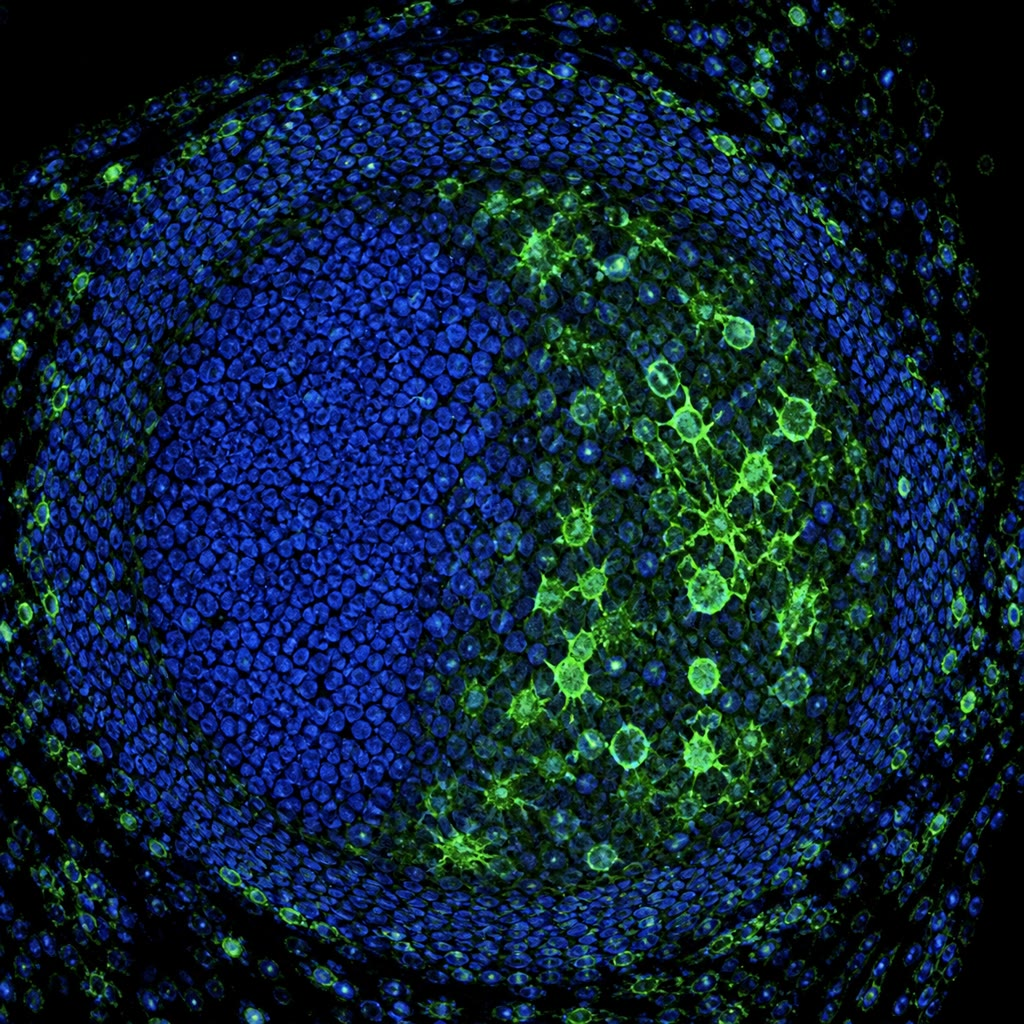
\includegraphics[width=0.36\linewidth]{images/book5/ai/b5-16-germinal-centre.jpg}\hspace{0.04\linewidth}
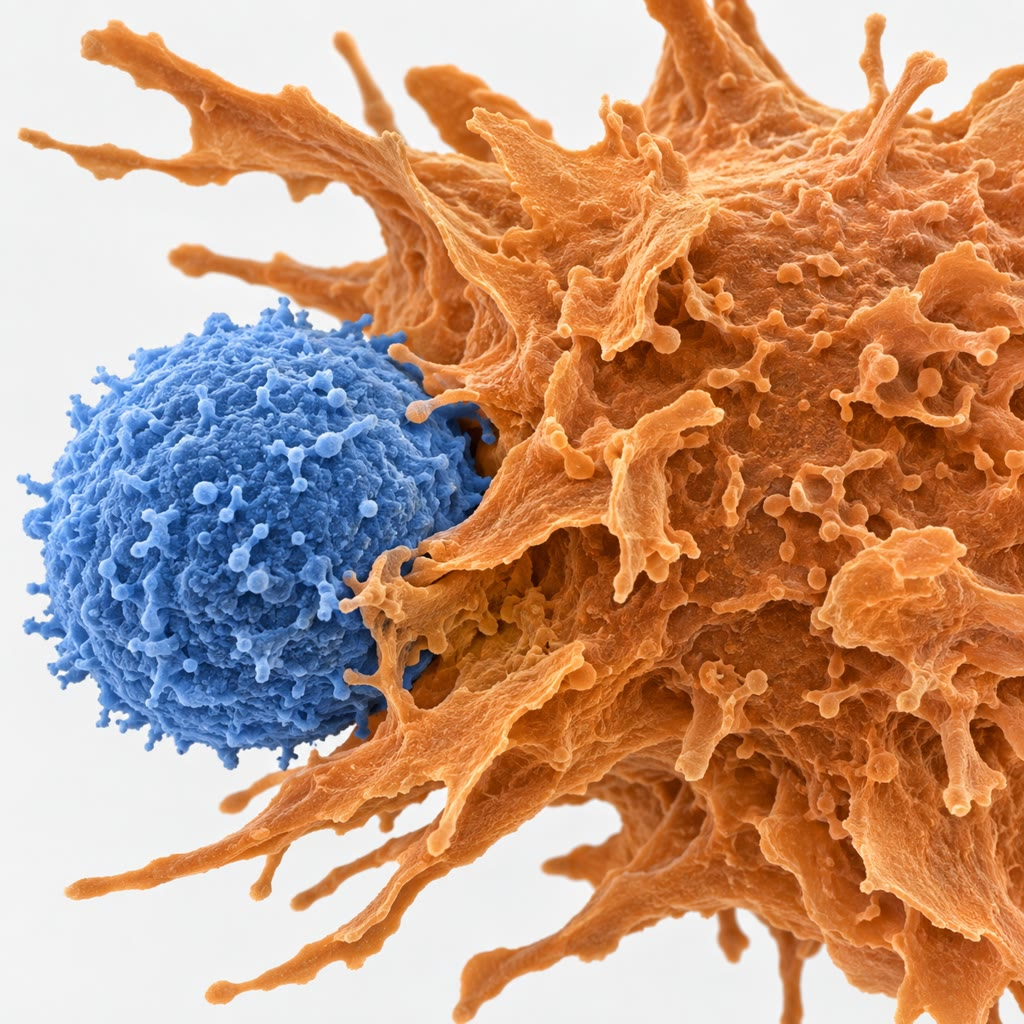
\includegraphics[width=0.36\linewidth]{images/book5/ai/b5-16-t-cell-apc.jpg}

{\small Links: een \omterm{def:b3:adaptive-immunity:germinal-centre}{kiemcentrum} in een \omterm{def:b3:adaptive-immunity:lymphocytes}{lymfeknoop} --- de dichtbevolkte
donkere zone en de lichtere zone van de selectie. Rechts: een \omterm{def:b3:adaptive-immunity:lymphocytes}{T-cel}
(klein) in contact met een \omterm{def:b3:innate-immunity:innate}{dendritische cel}, het ogenblik waarop de
adaptieve afweerreactie wordt beslist.}
\end{omfigure}

\section{Tolerantie en haar tekortkomingen}

\begin{definition}[Tolerantie]\label{def:b3:adaptive-immunity:tolerance}
\index{tolerantie}\index{negatieve selectie}\index{thymus}\index{anergie}\index{FoxP3}\index{auto-immuniteit}
Het repertoire wordt willekeurig gemaakt en bevat daarom receptoren
voor het eigen lichaam. \emph{Centrale tolerantie} verwijdert ze daar
waar de cellen rijpen: in de thymus worden T-cellen wier receptoren
eigen peptide--MHC te sterk binden gedood (\emph{negatieve selectie}),
worden ook de cellen gedood die MHC in het geheel niet kunnen binden
(zij zouden nutteloos zijn), en vertrekken alleen de enkele procenten
die ertussenin liggen; een transcriptiefactor, AIRE, laat cellen van de
thymus eiwitten uit elk weefsel tot expressie brengen --- insuline,
thyreoglobuline --- zodat T-cellen die daarvoor specifiek zijn daar
kunnen worden verwijderd. B-cellen die in het merg het eigen lichaam
binden worden verwijderd of herzien hun receptoren. \emph{Perifere
tolerantie} handelt de rest af: een \omterm{def:b3:adaptive-immunity:lymphocytes}{T-cel} die zijn \omterm{def:b3:adaptive-immunity:lymphocytes}{antigeen} zonder
\omterm{def:b3:adaptive-immunity:response}{co-stimulatie} ontmoet wordt onresponsief gemaakt (\emph{anergie}) of
verwijderd; en \emph{regulerende} T-cellen, bepaald door de factor
FoxP3, onderdrukken actief de reacties tegen het eigen lichaam en tegen
onschadelijke antigenen zoals voedsel en commensalen.
\emph{Auto-immuniteit} is het falen van deze controles: diabetes
type~1 (T-cellen vernietigen de $\beta$-cellen), multiple sclerose
(myeline), reumatoïde artritis (gewrichten), lupus (antilichamen tegen
kerncomponenten), schildklierziekte; elk daarvan hangt samen met
bepaalde HLA-allelen, die de betreffende eigen peptiden presenteren, en
sommige worden uitgelokt door besmetting met een microbe wier peptiden
op een eigen eiwit lijken (acuut reuma na een streptokokkeninfectie).
\end{definition}

\begin{proof}[Bewijsmateriaal]
Medawar (1953) spoot cellen van de ene ingeteelde muizenstam in
pasgeboren muizen van een andere; als volwassenen aanvaardden de
ontvangers huidtransplantaten van de donorstam die zij anders zouden
hebben afgestoten, terwijl zij transplantaten van derde stammen wel
afstootten. \omterm{def:b3:adaptive-immunity:tolerance}{Tolerantie} was verworven, specifiek, en vastgelegd door wat
het afweersysteem vroeg tegenkwam --- de proefondervindelijke grondslag
voor Burnets verwijdering van zelfreactieve klonen. Kinderen die zonder
een werkzaam AIRE-gen worden geboren ontwikkelen \omterm{def:b3:adaptive-immunity:tolerance}{auto-immuniteit} tegen
vele organen tegelijk; die zonder \omterm{def:b3:adaptive-immunity:tolerance}{FoxP3} (een zeldzaam X-gebonden
syndroom) ontwikkelen in hun eerste levensjaar een dodelijke
\omterm{def:b3:adaptive-immunity:tolerance}{auto-immuniteit} --- de twee armen van de \omterm{def:b3:adaptive-immunity:tolerance}{tolerantie}, elk aangetoond
door haar afwezigheid.
\end{proof}

\begin{example}[Overgevoeligheid, afweerstoornissen, transplantatie]\label{ex:b3:adaptive-immunity:failures}
\emph{Allergie} is een Th2-reactie op een onschadelijk \omterm{def:b3:adaptive-immunity:lymphocytes}{antigeen} ---
pollen, pinda, penicilline --- die IgE oplevert; bij hernieuwde
blootstelling verknoopt het \omterm{def:b3:adaptive-immunity:lymphocytes}{antigeen} het IgE op mestcellen, die binnen
minuten histamine vrijgeven, en zit het \omterm{def:b3:adaptive-immunity:lymphocytes}{antigeen} in het bloed, dan heet
die algemene vrijgave \emph{anafylaxie}, behandeld met adrenaline.
\emph{Afweerstoornissen}: kinderen zonder \omterm{def:b3:adaptive-immunity:antibody}{RAG} of zonder het enzym ADA
maken geen \omterm{def:b3:adaptive-immunity:lymphocytes}{lymfocyten} (ernstige gecombineerde immuundeficiëntie) en
sterven aan besmetting tenzij zij merg of gentherapie krijgen; hiv
vernietigt de CD4-T-cellen en daarmee de hulp die elke afweerreactie
nodig heeft. \emph{Transplantatie}: de T-cellen van de ontvanger zien
de HLA-moleculen van de donor als vreemd, en tot een tiende van alle
T-cellen antwoordt --- veel meer dan op enige ziekteverwekker --- zodat
transplantaten op de HLA-loci worden gematcht en de afweer van de
ontvanger levenslang wordt onderdrukt; een transplantaat van merg kan
omgekeerd zijn nieuwe gastheer aanvallen. En het doelbewuste gebruik:
de monoklonale antilichamen van \cref{ch:b3:genetic-engineering}, de
checkpointremmers die T-cellen tegen \omterm{def:b3:cancer-biology:hallmarks}{tumoren} loslaten
(\cref{ch:b3:cancer-biology}), en T-cellen die zijn uitgerust met een
chimere receptor voor een tumorantigeen (CAR-T), die leukemieën hebben
genezen waaraan niets anders raakte.
\end{example}

\section{Vaccinatie}

\begin{definition}[Vaccins en groepsimmuniteit]\label{def:b3:adaptive-immunity:vaccine}
\index{vaccin}\index{groepsimmuniteit}\index{basisreproductiegetal}\index{vaccinwerkzaamheid}
Een \emph{vaccin} biedt antigenen van een ziekteverwekker aan, met een
adjuvans of in een vorm die aangeboren receptoren prikkelt, zodat de
ontvanger \omterm{def:b3:adaptive-immunity:response}{geheugencellen} en antilichamen verwerft zonder de ziekte
(\cref{ch:b3:virology} somt de soorten op). Zijn \emph{werkzaamheid}
$E$ is het deel van de gevaccineerden dat beschermd is. De bescherming
reikt verder dan de gevaccineerden: een ziekteverwekker die zich
verspreidt in een bevolking waar elk geval gemiddeld $R_{0}$ anderen
besmet zolang allen vatbaar zijn --- het \emph{basisreproductiegetal}
--- besmet er nog maar $R_{0}$ maal het vatbare deel wanneer sommigen
immuun zijn, en sterft uit zodra dat getal onder één zakt. Dat is de
\emph{groepsimmuniteit}: boven een drempel van immune mensen breekt de
keten van overdracht en worden de niet-gevaccineerden --- zuigelingen,
mensen met een verzwakte afweer, en zij bij wie het vaccin faalde ---
door de anderen beschermd.
\end{definition}

\begin{theorem}[De drempel van de groepsimmuniteit]\label{thm:b3:adaptive-immunity:herd}
\index{groepsimmuniteit!drempel}\index{SIR-model}
In een bevolking waarin een deel $p$ immuun is en de rest vatbaar,
besmet elk geval gemiddeld $R_{\text{eff}} = R_{0}(1 -
p)$ anderen. Een epidemie kan niet beginnen als $R_{\text{eff}} < 1$,
dat wil zeggen als
\[
p > p_{c} = 1 - \frac{1}{R_{0}} .
\]
Met een \omterm{def:b3:adaptive-immunity:vaccine}{vaccin} van werkzaamheid $E$ is de benodigde dekkingsgraad
$f_{c} = p_{c}/E$. Loopt een epidemie wel in een vatbare bevolking (het
\omterm{thm:b3:adaptive-immunity:herd}{SIR-model}, met besmettingssnelheid $\beta$ en herstelsnelheid $\gamma$,
$R_{0} =
\beta/\gamma$), dan piekt zij wanneer het vatbare deel tot $1/R_{0}$ is
gedaald, en voldoet het deel dat nooit wordt besmet, $s_{\infty}$, aan
$\ln s_{\infty} = -R_{0}(1 - s_{\infty})$.
\end{theorem}
\begin{proof}
Elk geval legt contacten die $R_{0}$ mensen zouden besmetten als allen
vatbaar waren; een deel $1 - p$ van hen is dat, dus $R_{\text{eff}} =
R_{0}(1-p)$, en de voorwaarde $R_{\text{eff}} < 1$ geeft $p_{c}$; een
\omterm{def:b3:adaptive-immunity:vaccine}{vaccin} dat een deel $E$ van wie het krijgt beschermt, maakt een deel
$Ef$ van de bevolking immuun, dus $Ef > p_{c}$. In het \omterm{thm:b3:adaptive-immunity:herd}{SIR-model} geldt
$\mathrm{d}s/\mathrm{d}t = -\beta si$ en $\mathrm{d}i/\mathrm{d}t =
\beta si - \gamma i = \gamma i(R_{0}s - 1)$, dus groeit $i$ zolang $s >
1/R_{0}$ en daalt daarna: de piek ligt bij $s = 1/R_{0}$. Deling van de
twee vergelijkingen geeft $\mathrm{d}i/\mathrm{d}s = -1 + 1/(R_{0}s)$,
dus is $i + s -
\ln s/R_{0}$ constant; berekend aan het begin ($s = 1$, $i
\approx 0$) en aan het eind ($i = 0$, $s = s_{\infty}$) levert dat
$s_{\infty} - \ln s_{\infty}/R_{0} = 1$ op, de relatie voor de
einduitkomst.
\end{proof}

\begin{example}[Mazelen en pokken]\label{ex:b3:adaptive-immunity:measles}
Mazelen hebben $R_{0} \approx 15$: $p_{c} = 1 - 1/15 = 93\,\%$, en met
een \omterm{def:b3:adaptive-immunity:vaccine}{vaccin} met een werkzaamheid van $97\,\%$ na twee doses is de
benodigde dekkingsgraad $96\,\%$ --- daarom keren de mazelen terug
overal waar de vaccinatie een paar procent verslapt, en daarom is een
niet-gevaccineerd kind in een goed gevaccineerd land toch veilig.
Pokken hadden $R_{0} \approx 5$--$7$, een drempel rond $80$--$85\,\%$,
geen dierlijk reservoir, geen symptoomloze dragers en een \omterm{def:b3:adaptive-immunity:vaccine}{vaccin} dat in
één dosis werkte: uitroeibaar, en uitgeroeid. Polio is er bijna. Griep
en de coronavirussen, wier antigenen verschuiven
(\cref{ch:b3:virology}) en wier immuniteit wegebt, zijn dat niet. In
een niet-gevaccineerde bevolking besmet een epidemie met $R_{0} = 3$,
volgens de relatie voor de einduitkomst, $1 - s_{\infty} = 94\,\%$ van
de mensen; met $R_{0} = 1.5$, $58\,\%$.
\end{example}

\begin{omfigure}
\begin{tikzpicture}
\begin{axis}[
  width=6.4cm, height=5.4cm,
  axis x line=bottom, axis y line=left,
  xmin=1, xmax=18, ymin=0, ymax=1,
  xlabel={$R_{0}$}, ylabel={drempel $p_{c}$},
  xlabel style={font=\small, at={(axis description cs:0.5,-0.12)}, anchor=north}, ylabel style={font=\small},
  tick label style={font=\scriptsize}, xtick={1,3,6,9,12,15,18}, ytick={0,0.5,0.8,0.93,1}, yticklabels={0,0.5,0.8,0.93,1},
  clip=false,
]
\addplot[very thick, omDef, domain=1:18, samples=80] {1-1/x};
\fill[omThm] (axis cs:15,0.933) circle (2pt); \node[font=\scriptsize, anchor=south east] at (axis cs:15,0.94) {mazelen};
\fill[omThm] (axis cs:6,0.833) circle (2pt); \node[font=\scriptsize, anchor=north west] at (axis cs:6.3,0.82) {pokken};
\fill[omThm] (axis cs:2.5,0.6) circle (2pt); \node[font=\scriptsize, anchor=north west] at (axis cs:2.6,0.58) {griep van 1918};
\end{axis}
\begin{axis}[
  at={(7.6cm,0)}, anchor=south west,
  width=6.4cm, height=5.4cm,
  axis x line=bottom, axis y line=left,
  xmin=0, xmax=60, ymin=0, ymax=0.35,
  xlabel={dagen}, ylabel={besmettelijk deel},
  xlabel style={font=\small, at={(axis description cs:0.5,-0.12)}, anchor=north}, ylabel style={font=\small},
  tick label style={font=\scriptsize}, xtick={0,20,40,60}, ytick={0,0.1,0.2,0.3},
  clip=false,
]
\addplot[very thick, omThm, smooth] coordinates {(0,0.001) (5,0.003) (10,0.012) (15,0.04) (20,0.12) (25,0.25) (28,0.30) (31,0.27) (35,0.18) (40,0.09) (45,0.04) (50,0.015) (55,0.006) (60,0.002)};
\addplot[very thick, omDef, smooth] coordinates {(0,0.001) (5,0.0015) (10,0.0025) (15,0.004) (20,0.006) (25,0.009) (30,0.012) (35,0.014) (40,0.015) (45,0.014) (50,0.012) (55,0.009) (60,0.007)};
\node[font=\scriptsize, omThm, anchor=west] at (axis cs:30,0.3) {geen immuniteit, $R_{0} = 3$};
\node[font=\scriptsize, omDef, anchor=south west] at (axis cs:32,0.03) {\qty{60}{\%} gevaccineerd: $R_{\text{eff}} = 1.2$};
\end{axis}
\end{tikzpicture}

{\small Links: de drempel $1 - 1/R_{0}$ --- hoe besmettelijker de
ziekte, hoe dichter bij iedereen immuun moet zijn. Rechts: een
SIR-epidemie met $R_{0} = 3$ in een naïeve bevolking en in een
bevolking waarvan \qty{60}{\%} immuun is, wat niet genoeg is om haar te
stoppen maar haar wel afvlakt en vertraagt.}
\end{omfigure}

\begin{omfigure}
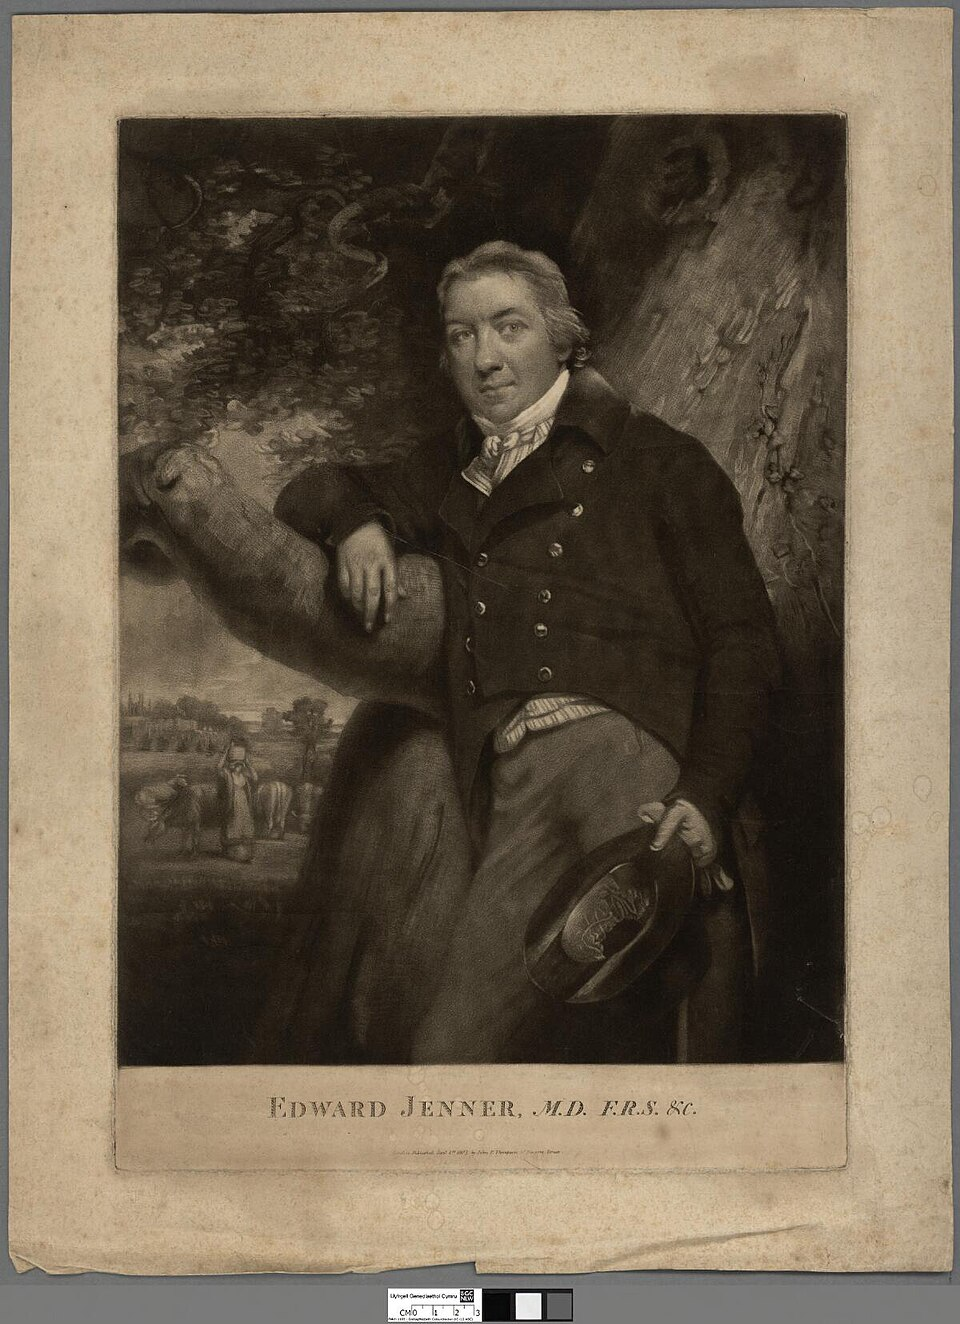
\includegraphics[width=0.30\linewidth]{images/book5/jenner.jpg}\hspace{0.04\linewidth}
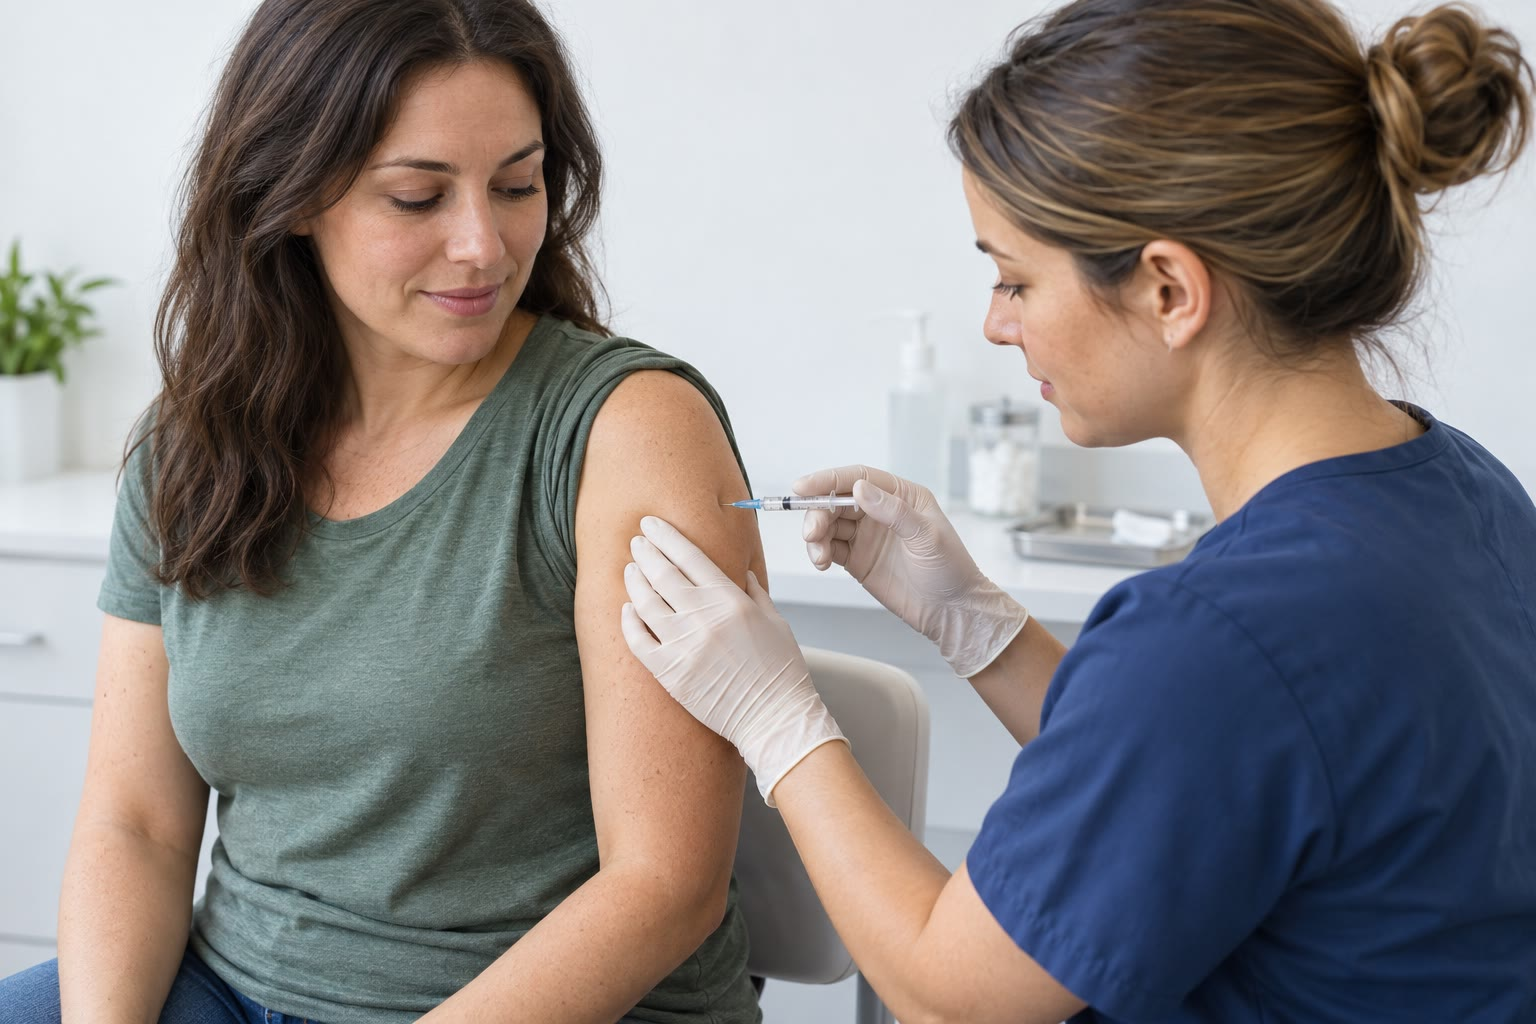
\includegraphics[width=0.50\linewidth]{images/book5/ai/b5-16-vaccination.jpg}

{\small Edward Jenner, die in 1796 een jongen met koepokken tegen de
pokken beschermde en zo de vaccinatie stichtte (gravure uit 1807,
publiek domein). Rechts: dezelfde handeling twee eeuwen later --- een
intramusculair \omterm{def:b3:adaptive-immunity:vaccine}{vaccin}, waarvan de \omterm{def:b3:innate-immunity:innate}{dendritische cellen} van de deltaspier
het \omterm{def:b3:adaptive-immunity:lymphocytes}{antigeen} naar de okselklieren zullen dragen.}
\end{omfigure}

\begin{remark}[Wat de afweer onthoudt]\label{rem:b3:adaptive-immunity:memory}
Het adaptieve afweersysteem is een darwiniaanse machine in ieder van
ons: willekeurige variatie (V(D)J, hypermutatie), selectie (door
\omterm{def:b3:adaptive-immunity:lymphocytes}{antigeen}, in het \omterm{def:b3:adaptive-immunity:germinal-centre}{kiemcentrum}, tegen het eigen lichaam in de \omterm{def:b3:adaptive-immunity:tolerance}{thymus}) en
overerving (\omterm{def:b3:adaptive-immunity:response}{geheugencellen}, klonale uitbreiding). Het lost in weken het
probleem op dat de evolutie in millennia oplost --- een molecuul dat
een nooit eerder gezien doelwit bindt --- en zijn antwoorden behoren
tot de best bestudeerde gevallen van rechtstreeks waargenomen evolutie.
Zijn prijs is \omterm{def:b3:adaptive-immunity:tolerance}{auto-immuniteit}, zijn afhankelijkheid van het oordeel van
het aangeboren systeem is volstrekt, en zijn geheugen, dat Jenner
benutte en dat \omterm{def:b3:adaptive-immunity:vaccine}{vaccins} doelbewust beschrijven, is de reden dat een
soort van langlevende, traag voortplantende dieren kan overleven in een
wereld van snel voortplantende microben.
\end{remark}

\section{Opgaven}

\begin{exercise}[$\star$]\label{exo:b3:adaptive-immunity:1}
Noem de vier stellingen van de \omterm{def:b3:adaptive-immunity:lymphocytes}{klonale selectie} en het experiment dat
elk van de eerste twee steunt.
\end{exercise}

\begin{exercise}[$\star$]\label{exo:b3:adaptive-immunity:2}
Beschrijf de bouw van een \omterm{def:b3:adaptive-immunity:antibody}{antilichaam} en geef de functie van elk van de
vijf klassen.
\end{exercise}

\begin{exercise}[$\star$]\label{exo:b3:adaptive-immunity:3}
Zet \omterm{def:b3:adaptive-immunity:mhc}{MHC-klasse~I} en klasse~II tegenover elkaar naar celverdeling,
herkomst van het peptide, peptidelengte en de \omterm{def:b3:adaptive-immunity:lymphocytes}{T-cel} die elk afleest.
\end{exercise}

\begin{exercise}[$\star$]\label{exo:b3:adaptive-immunity:4}
Definieer $R_{0}$ en de drempel van de \omterm{def:b3:adaptive-immunity:vaccine}{groepsimmuniteit}, en bereken de
drempel voor de bof ($R_{0} = 5$), kinkhoest ($R_{0} = 12$) en de griep
van 1918 ($R_{0} = 2.5$).
\end{exercise}

\begin{exercise}[$\star\star$]\label{exo:b3:adaptive-immunity:5}
Een soort heeft $V_{H} = 50$, $D = 20$, $J_{H} = 5$ en één lichte locus
met $V = 60$, $J = 4$. Bereken het combinatorische repertoire en
vervolgens het totaal met een junctionele factor $10^{4}$. Hoe
verhoudt dat zich tot de $10^{9}$ B-cellen die het dier heeft?
\end{exercise}

\begin{exercise}[$\star\star$]\label{exo:b3:adaptive-immunity:6}
Het variabele gebied van een \omterm{def:b3:adaptive-immunity:lymphocytes}{B-cel} in een \omterm{def:b3:adaptive-immunity:germinal-centre}{kiemcentrum} telt
\qty{1000}{bp}; AID muteert met $10^{-3}$ per basepaar per deling.
Hoeveel mutaties per cel over $20$ delingen, en hoeveel verschillende
varianten van het \omterm{def:b3:adaptive-immunity:antibody}{antilichaam} met één gewisselde base ontstaan er onder
$10^{5}$ cellen? Vergelijk met de $3000$ mogelijke enkelvoudige
substituties.
\end{exercise}

\begin{exercise}[$\star\star$]\label{exo:b3:adaptive-immunity:7}
Leg uit waarom een \omterm{def:b3:adaptive-immunity:lymphocytes}{T-cel} van de ene mens geen virale peptiden herkent
die door de cellen van een ander worden gepresenteerd, en waarom
datzelfde feit transplantaties moeilijk maakt en het HLA-systeem
polymorf.
\end{exercise}

\begin{exercise}[$\star\star$]\label{exo:b3:adaptive-immunity:8}
Voorspel het afweerfenotype van een kind zonder (a) RAG1, (b) AIRE,
(c) \omterm{def:b3:adaptive-immunity:tolerance}{FoxP3}, (d) het klassenwisselingsenzym AID, en (e) CD4-T-cellen.
\end{exercise}

\begin{exercise}[$\star\star$]\label{exo:b3:adaptive-immunity:9}
Een \omterm{def:b3:adaptive-immunity:vaccine}{vaccin} heeft een werkzaamheid van \qty{90}{\%} en de ziekte
$R_{0} = 6$. Welke dekkingsgraad stopt de overdracht? Wat is bij een
dekkingsgraad van \qty{80}{\%} de waarde van $R_{\text{eff}}$, en welk
deel van de bevolking besmet een epidemie (gebruik de relatie voor de
einduitkomst met $R_{0}$ vervangen door $R_{\text{eff}}$ onder de
vatbaren --- of beredeneer waarom dat bij benadering juist is)?
\end{exercise}

\begin{exercise}[$\star\star\star$]\label{exo:b3:adaptive-immunity:10}
Leid de relatie voor de einduitkomst uit de stelling af uit de
SIR-vergelijkingen en los haar numeriek op voor $R_{0} = 1.5$, $2$, $3$
en $5$. Waarom besmet een epidemie nooit iedereen, zelfs zonder enige
ingreep?
\end{exercise}

\begin{exercise}[$\star\star\star$]\label{exo:b3:adaptive-immunity:11}
\omterm{def:b3:adaptive-immunity:germinal-centre}{Affiniteitsrijping} verhoogt de binding in drie weken duizendvoudig.
Behandel het \omterm{def:b3:adaptive-immunity:germinal-centre}{kiemcentrum} als een populatie onder selectie: bij een
mutatietempo van één per cel per deling, met een deel $10^{-2}$ van de
mutaties dat de affiniteit met een factor $1.5$ verbetert en de rest
neutraal of schadelijk, hoeveel selectieronden zijn er nodig voor een
duizendvoudige winst, en hoeveel cellen moet elke ronde doorzoeken?
Bespreek waarom het \omterm{def:b3:adaptive-immunity:germinal-centre}{kiemcentrum} in cycli is georganiseerd.
\end{exercise}

\begin{exercise}[$\star\star\star$]\label{exo:b3:adaptive-immunity:12}
Auto-immuunziekten komen vaker voor bij vrouwen en hangen samen met
HLA-allelen; diabetes type~1 is in rijke landen in vijftig jaar
vervijfvoudigd. Stel, met de mechanismen van dit hoofdstuk en van
\cref{ch:b3:microbiomes}, verklaringen voor elke waarneming voor en één
toets van elke verklaring.
\end{exercise}

\section{Vraagstuk: een vaccinatiecampagne}

\begin{problem}[{Weekendvraagstuk --- een repertoire geteld, een
afweerreactie geklokt van honderd cellen tot een milliliter serum, een
kiemcentrum uitgevoerd als evolutionair algoritme, en een
mazelencampagne gepland tegen de groepsdrempel, eindigend bij de omvang
van het repertoire, het antilichaam dat een plasmacel op een dag maakt
en de dekkingsgraad die een land nodig heeft}]
\label{pb:b3:adaptive-immunity:1}
Gegevens: $V_{H} = 40$, $D = 25$, $J_{H} = 6$; lichte loci $(40, 5)$ en
$(30, 4)$; junctionele factor $3\times 10^{4}$. Een lichaam heeft
$10^{11}$ B-cellen; één op $10^{5}$ bindt een gegeven epitoop; $100$
voorlopers worden gerekruteerd; deling elke \qty{8}{h} gedurende $7$
dagen; \qty{30}{\%} van de kloon wordt \omterm{def:b3:adaptive-immunity:response}{plasmacel}, elk met een
uitscheiding van $2000$ IgG-moleculen per seconde; IgG weegt
\qty{150}{kDa}; plasmavolume \qty{3}{L}; halveringstijd van IgG
\qty{21}{d}. \omterm{def:b3:adaptive-immunity:germinal-centre}{Kiemcentrum}: variabel gebied van \qty{1000}{bp}, $10^{-3}$
mutaties per bp per deling, één op $100$ mutaties verbetert de
affiniteit met $1.5$. Mazelen: $R_{0} = 15$, \omterm{def:b3:adaptive-immunity:vaccine}{vaccinwerkzaamheid} $0.93$
na één dosis en $0.97$ na twee; een land van $5\times 10^{6}$ inwoners
met $60\,000$ geboorten per jaar.

\medskip
\noindent\textbf{Deel I --- Het repertoire.}
\begin{enumerate}
  \item Bereken het combinatorische repertoire en het totaal met
        \omterm{def:b3:adaptive-immunity:antibody}{junctionele diversiteit}.
  \item Vergelijk met het aantal B-cellen. Welk deel van het mogelijke
        repertoire brengt één lichaam tegelijk tot expressie, en wat
        volgt daaruit voor de repertoires van twee individuen?
  \item Hoeveel B-cellen in het lichaam binden het epitoop? Hoeveel
        gemiddeld in een \omterm{def:b3:adaptive-immunity:lymphocytes}{lymfeknoop} met $10^{8}$ B-cellen?
  \item Een pasgeborene heeft $10^{9}$ B-cellen. Hoeveel binden het
        epitoop, en waarom is de reactie van een pasgeborene toch zwak?
  \item De derde lus van de zware keten van een \omterm{def:b3:adaptive-immunity:antibody}{antilichaam} ontstaat
        door \omterm{def:b3:adaptive-immunity:antibody}{junctionele diversiteit}. Leg uit waarom deze lus het meest
        variabele deel van het molecuul is en meestal in het midden van
        de bindingsplaats ligt.
  \item \omterm{def:b3:adaptive-immunity:germinal-centre}{Somatische hypermutatie} voegt diversiteit toe na de selectie,
        V(D)J ervoor. Waarom is het voordelig beide te hebben, in die
        volgorde?
\end{enumerate}

\medskip
\noindent\textbf{Deel II --- De afweerreactie.}
\begin{enumerate}[resume]
  \item Uitgaande van $100$ cellen die elke \qty{8}{h} delen, hoeveel
        zijn er na $7$ dagen? Hoeveel \omterm{def:b3:adaptive-immunity:response}{plasmacellen}?
  \item Hoeveel IgG-moleculen scheiden zij per dag uit, en welke massa?
        Welke serumconcentratie geeft de opbrengst van één dag in
        \qty{3}{L}?
  \item Wat is na tien dagen uitscheiding op dat tempo, zonder rekening
        te houden met afbraak, de concentratie in g/L? Vergelijk met
        het normale totale IgG van \qty{10}{g/L}.
  \item De \omterm{def:b3:adaptive-immunity:response}{plasmacellen} sterven na twee weken; het \omterm{def:b3:adaptive-immunity:antibody}{antilichaam} vervalt
        daarna met een halveringstijd van \qty{21}{d}. Hoe lang duurt
        het voordat de concentratie van vraag 9 honderdvoudig daalt?
        Wat houdt \omterm{def:b3:adaptive-immunity:antibody}{antilichaam} jarenlang in stand?
  \item Een secundaire afweerreactie begint bij $10^{5}$
        \omterm{def:b3:adaptive-immunity:response}{geheugencellen}. Hoeveel cellen na $3$ dagen, en hoe verhoudt
        zich dat tot de primaire reactie op dag 3 en dag 7?
  \item Leg uit waarom in een primaire reactie IgM het eerst komt en
        IgG later, en waarom de secundaire reactie van meet af aan IgG
        is.
\end{enumerate}

\medskip
\noindent\textbf{Deel III --- Het \omterm{def:b3:adaptive-immunity:germinal-centre}{kiemcentrum}.}
\begin{enumerate}[resume]
  \item Hoeveel mutaties krijgt een \omterm{def:b3:adaptive-immunity:lymphocytes}{B-cel} per deling in haar variabele
        gebied? En over $20$ delingen?
  \item Welk deel van de dochtercellen van één deling draagt een
        verbeterende mutatie? Hoeveel verbeterde cellen verschijnen er
        per deling in een \omterm{def:b3:adaptive-immunity:germinal-centre}{kiemcentrum} van $10^{4}$ delende cellen?
  \item Hoeveel opeenvolgende verbeteringen met $1.5$ geven een
        duizendvoudige winst in affiniteit? Als elke selectieronde twee
        delingen duurt (\qty{12}{h}), hoe lang is dat?
  \item De meeste mutaties beschadigen het \omterm{def:b3:adaptive-immunity:antibody}{antilichaam}. Als
        \qty{50}{\%} van de mutaties de binding vernietigt, welk deel
        van de cellen overleeft de mutatie van elke deling, en waarom
        moet de lichte zone de meeste cellen doden?
  \item Een \omterm{def:b3:adaptive-immunity:vaccine}{vaccin} dat in twee doses met zes weken tussentijd wordt
        gegeven levert antilichamen met een hogere affiniteit op dan
        één dosis. Verklaar dat met het \omterm{def:b3:adaptive-immunity:germinal-centre}{kiemcentrum}.
  \item Sommige virussen (hiv, griep) ontsnappen aan antilichamen door
        hun oppervlak te muteren. Leg uit waarom het \omterm{def:b3:adaptive-immunity:germinal-centre}{kiemcentrum} toch
        de grondslag is voor de hoop op een breed beschermend \omterm{def:b3:adaptive-immunity:vaccine}{vaccin}.
\end{enumerate}

\medskip
\noindent\textbf{Deel IV --- De campagne.}
\begin{enumerate}[resume]
  \item Groepsdrempel voor mazelen, en de vereiste dekkingsgraad bij
        één dosis; bij twee doses.
  \item Het land vaccineert \qty{90}{\%} van de kinderen met twee
        doses. Immuun deel, $R_{\text{eff}}$, en het oordeel:
        circuleren de mazelen?
  \item Hoeveel vatbare kinderen stapelen zich per geboortejaar op bij
        een dekkingsgraad van \qty{90}{\%} (niet-gevaccineerden plus
        vaccinfalen)? Hoeveel vatbaren zijn er na vijf jaar zonder
        mazelen, en waarom veroorzaakt een invoer dan een uitbraak?
  \item Schat met de relatie voor de einduitkomst en het effectieve
        reproductiegetal onder de vatbaren welk deel van die vatbaren
        een uitbraak besmet. (Neem $R_{\text{eff}}$ uit vraag 20 als
        het reproductiegetal in de hele bevolking, en merk op dat de
        ziekte zich binnen de vatbare groep verspreidt alsof $R_{0}$
        gelijk was aan $R_{\text{eff}}$.)
  \item De dekkingsgraad wordt met twee doses op \qty{95}{\%} gebracht.
        Immuun deel en $R_{\text{eff}}$; is de drempel gehaald?
  \item Zuigelingen onder één jaar kunnen niet tegen mazelen worden
        gevaccineerd en sterven er het vaakst aan. Leg uit hoe de
        campagne hen beschermt, en wat er met hun bescherming gebeurt
        als de dekkingsgraad tot \qty{85}{\%} zakt.
  \item Vat samen: het totale repertoire (vraag~1), het IgG dat de
        \omterm{def:b3:adaptive-immunity:response}{plasmacellen} van één dag maken (vraag~8), en de dekkingsgraad
        met twee doses die het land nodig heeft (vraag~19).
\end{enumerate}
\end{problem}
